\documentclass[10pt,a4paper,sans]{article}
\usepackage{dirtytalk}
\usepackage{amsmath}
\usepackage{graphicx}
\graphicspath{ {image/} }

\begin{document}

\section{Abstract}

\begin{itemize}
   \item{Abstract: high throughput sequencing is not unbiased. It is definitely more comprehensive than microarrays.}
\end{itemize}

\noindent
I have re-worded the original sentence:
\\\\
\say{Traditionally, transcriptome profiling has relied on microarray technologies but with the advent of high-throughput sequencing, the ability to profile transcripts accurately and in an unbiased manner has transformed the study of transcriptomes. However the applications of high-throughput sequencing to transcriptomics is relatively immature as developments have occurred in the last 5-6 years.}
\\\\
into
\\\\
\say{Traditionally, transcriptome profiling has relied on microarray technologies but with the advent of high-throughput transcriptome sequencing, transcripts can be profiled without \textit{a priori} knowledge of their sequence and their expression levels can be digitally measured. This has transformed the field of transcriptomics, however the applications of high-throughput sequencing to transcriptomics is relatively immature as developments have occurred in the last 5-6 years.}

\begin{itemize}
   \item{Abstract: last sentence needs rephrasing}
\end{itemize}

\noindent
I have re-worded the final paragraph of the abstract from:
\\\\
\say{The layers of complexity include the expression of multiple classes of RNA species, each performing various regulatory roles, random transcriptional events or transcriptional noise, and complexity perpetrated from technical artefacts. In order to separate noise from signal requires an understanding of the different technologies, careful scrutiny of the data, and the application of appropriate bioinformatic methods.}
\\\\
into
\\\\
\say{The interpretation of this complexity has been a highly controversial topic; on one end of the spectrum, is the theory that the majority of the genome is functional, and on the other end is the counter-argument that most of the genome produces non-functional products. An important point raised from this discussion was that simply observing a transcription event is not enough evidence for function. Transcriptional signal may come from the expression of various classes of RNA species, or from random transcription events and technical artefacts. It is important to keep these considerations in mind when analysing eukaryotic transcriptomic data sets.}

\begin{itemize}
   \item{Nederlandse samenvatting: tissue into weefsel}
\end{itemize}

\noindent
I have re-worded the Dutch summary from:
\\\\
\say{$\dots$ waarbij hun expressie tissue specifiek is.}
\\\\
into
\\\\
\say{$\dots$ waarbij hun expressie weefsel specifiek is.}

\section{Chapter 1}

\begin{itemize}
   \item{The description of SAGE is a bit inaccurate as the sequences in the early SAGE method were indeed always 9-10 bp long but the tag is usually said to also contain the restriction enzyme site so the total length is 13-14 and therefore better able to discriminate transcripts than a 9-10 bp tag. Also, the tag is not at the ultimate 3’-end as the text suggests.}
\end{itemize}
\noindent
In the thesis I wrote:
\\\\
\say{A technology called Serial Analysis of Gene Expression (SAGE) was the first tag-based approach, which created 9 to 10 bp long tags that generally corresponded to the 3' end of the transcripts.}
\\\\
This was based on what I read in Velculescu et al. 1995, which I quote:
\\\\
\say{SAGE is based on two principles. First, a short nucleotide sequence tag [9 to 10 base pairs (bp)] contains sufficient information to uniquely identify a transcript $\dots$}
\\\\
I had a look at the schematic of SAGE, and of course you are correct; the restriction site is also included in the tag. However, throughout the entire paper they only referred to the 9 bp length; I guess since they could associate 95\% of the 9 bp tags to GenBank transcripts, they did not need the extra 4 bps? You are also correct about the 3' end. I have modified the sentence to:
\\\\
\say{A technology called Serial Analysis of Gene Expression (SAGE) was the first tag-based approach, which created 13 to 14 bp long tags (including the restriction site of the anchoring enzyme). These tags corresponded to the most 3' portion of a cDNA where a restriction site for the anchoring enzyme would be present.}

\begin{itemize}
   \item{The CAGE figure could be clearer. Currently it is not clear that only capped RNAs are measured, and it is not clear the endonuclease cuts downstream of its recognition site.}
\end{itemize}

\noindent
I have modified the image and the caption as follows:

\begin{figure}[!ht]
   \centering
   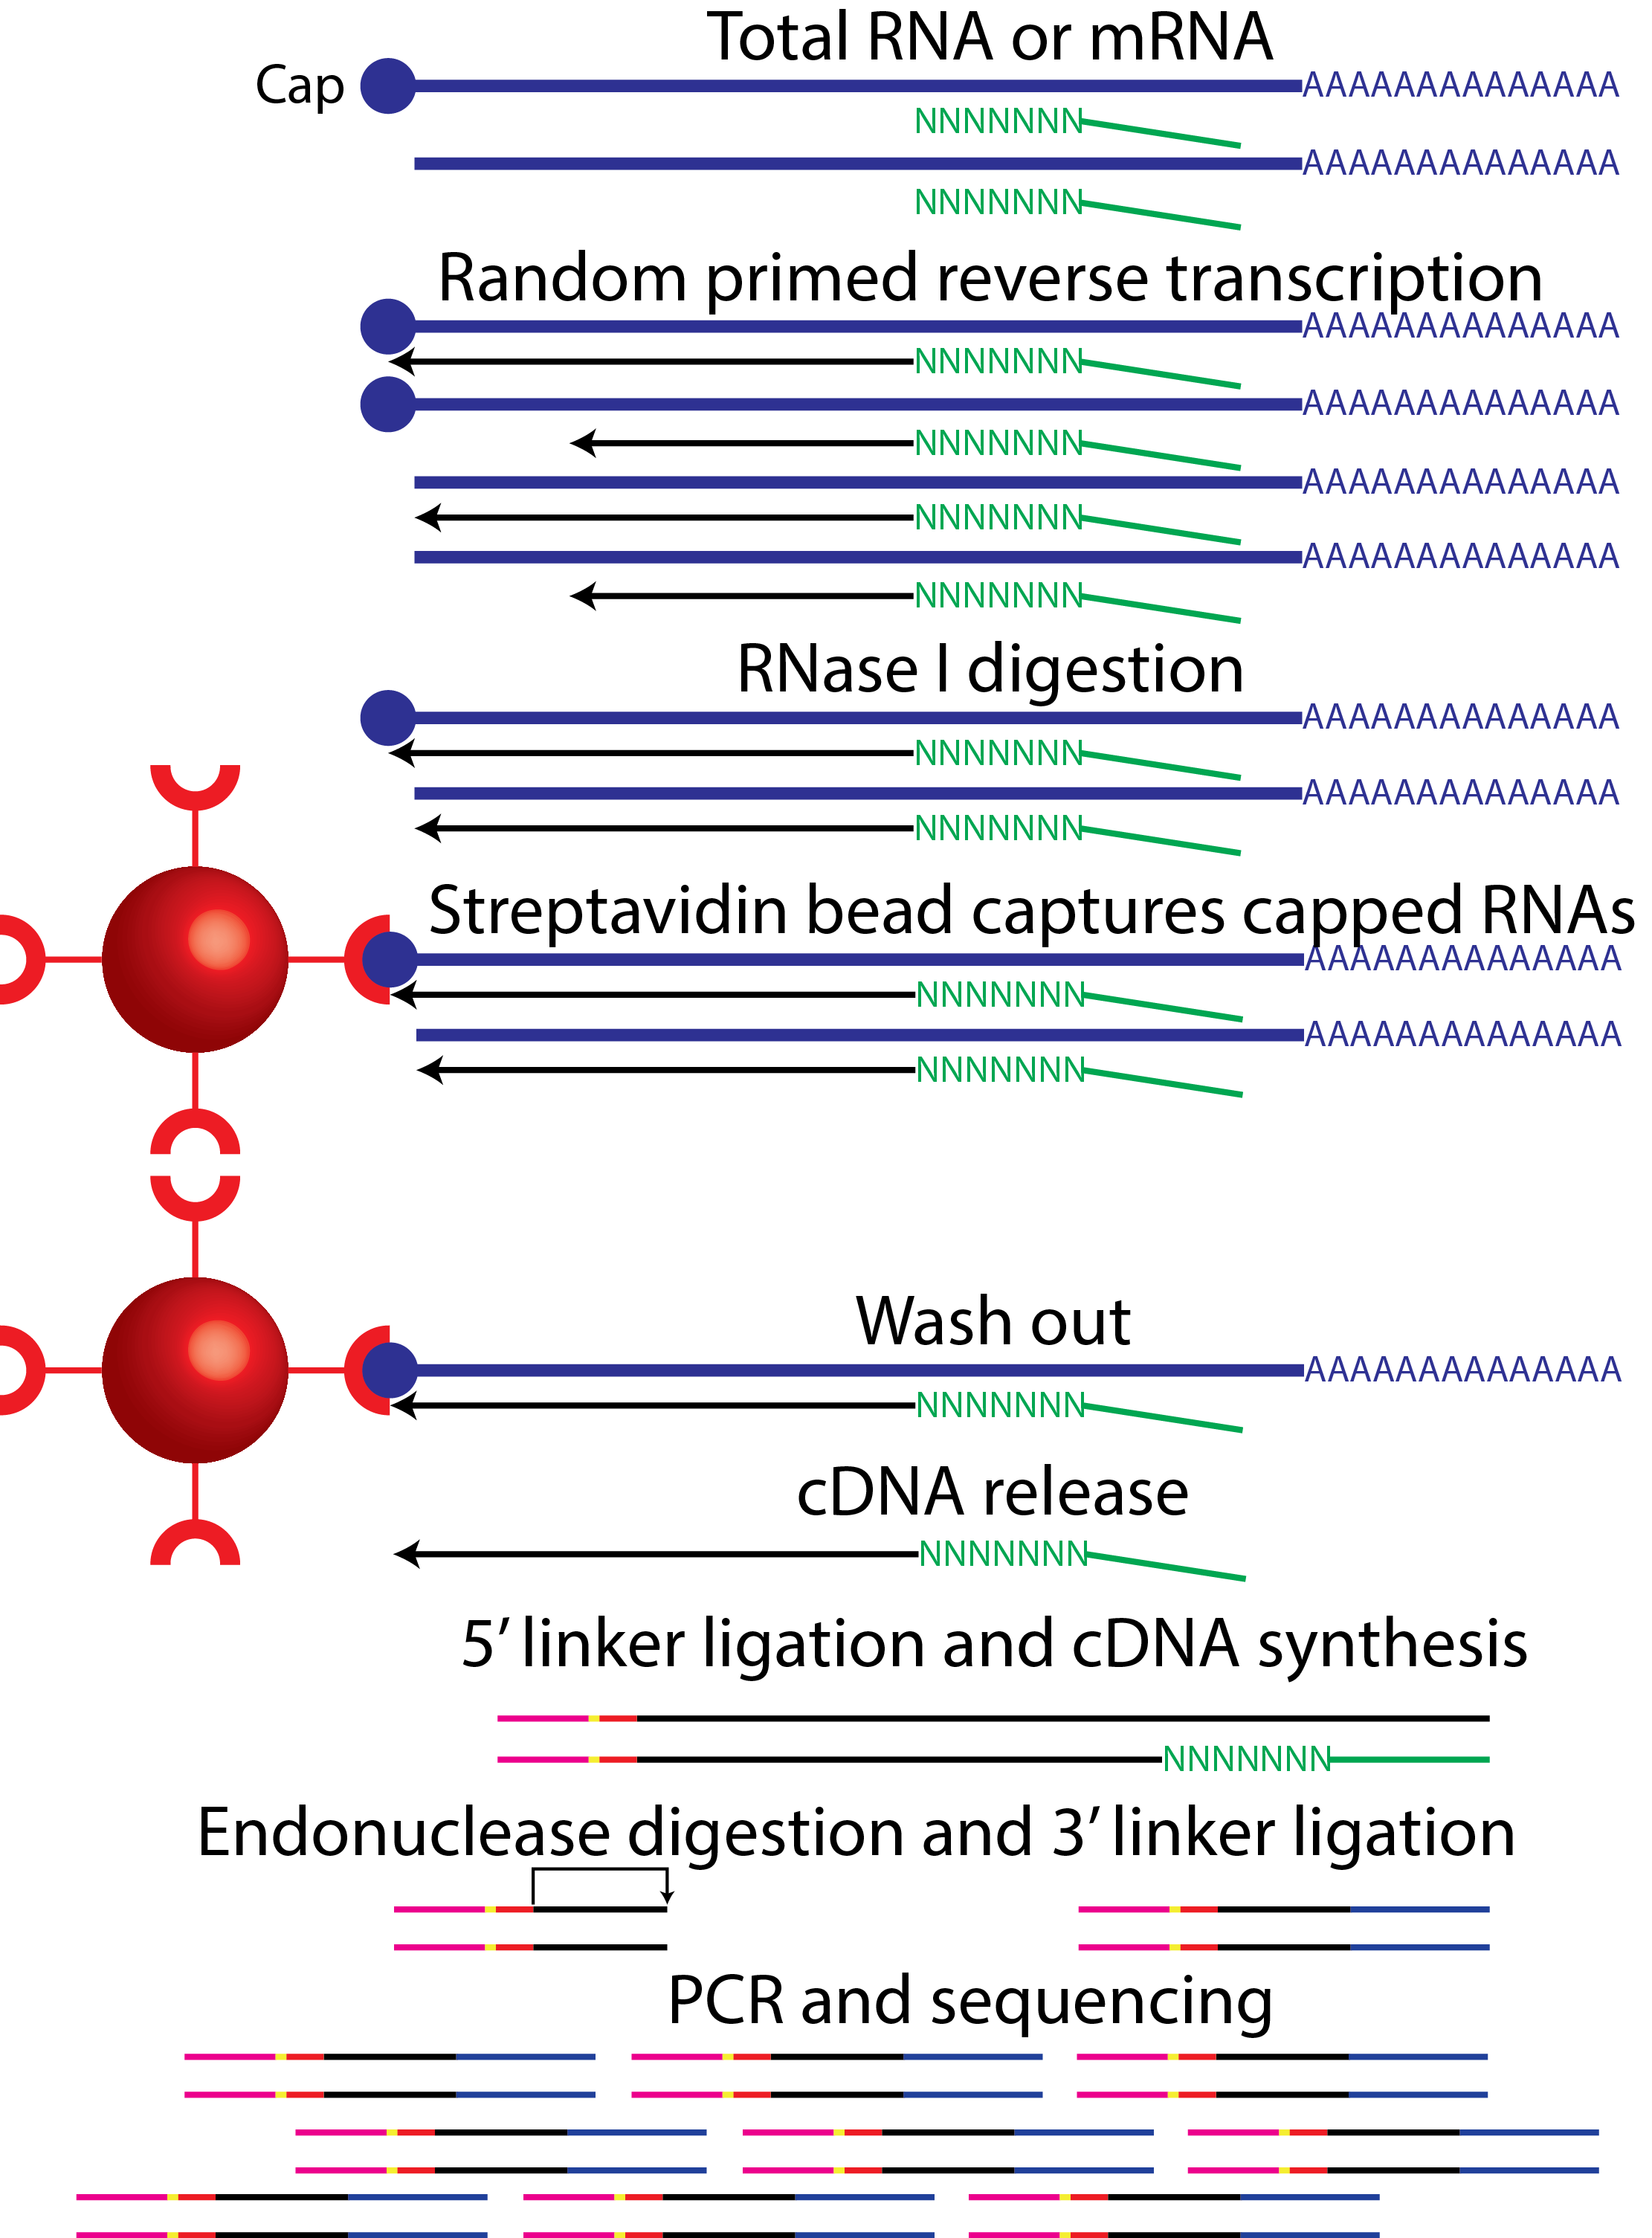
\includegraphics[width=\textwidth,natwidth=2254,natheight=3051,totalheight=0.65\textheight,keepaspectratio]{cage_protocol.png}
   \caption[Cap Analysis Gene Expression protocol]{\small The tagging Cap Analysis Gene Expression (CAGE) protocol starts with synthesising cDNA from either total RNA or mRNA by using random or oligo dT primers (only random primers are shown here). Reverse transcription takes place in RNAs with or without a cap and to full or partial completion; the RNase I digestion step removes partially reverse transcribed RNA as they are not protected by a full double strand. The 5' end of cDNAs are selected by streptavidin beads that capture the biotin labelled cap structure and unbound cDNA are washed out. After release from the bead, a linker is attached to the 5' end of the single-stranded cDNA; this linker contains a barcode sequence (in yellow) followed by a recognition site (in red) that allow the endonuclease digestion. Lastly a linker is ligated to the 3' end of the tag sequence (in blue), which is amplified and directly sequenced.}
\end{figure}

\newpage

\begin{itemize}
   \item{Section 1.5.4: spliceosomal RNAs aid protein translation?}
\end{itemize}
\noindent
I have re-worded the original sentence:
\\\\
\say{Historically, it was believed that there were only a few ncRNA families, such as the tRNAs, rRNAs, and the spliceosomal RNAs, all of which aided protein translation.}
\\\\
into
\\\\
\say{Historically, it was believed that there were only a few ncRNA families, such as the tRNAs, rRNAs, and the spliceosomal RNAs, all of which aided the processing of proteins.}

\begin{itemize}
   \item{Section 1.8: the research goal is very broad. It would be good to set a few more specific goals related to the different chapters}
\end{itemize}
\noindent
I agree that the research goals were too broad. I will give this much more thought and update the goals.

\section{Chapter 3}

\begin{itemize}
   \item{I would advise to include supplementary data files. For example: Suppl Figures 22 and 23 are probably key figures for Chapter 3 generated by Dave but not included in the thesis.}
\end{itemize}
\noindent
I have now included supplementary figure 22 and 23 into the thesis.

\section{Chapter 5}

\begin{itemize}
   \item{I miss a discussion on the non-capped RNAs that may also be. I also miss whether you observe clear CAGE peaks / start sites for these lncRNAs (like for protein-coding RNAs) or multiple distinct start sites or an even more even coverage pattern.}
\end{itemize}

\noindent
I apologise for the incomplete chapter; I was in a hurry to compile the thesis and included a very rough draft of the manuscript, which I am still working on. I am more than happy to send you an updated version of the manuscript once I have it ready. To briefly answer your questions, there are instances of sharp transcription start sites (TSSs) and coverage like TSS patterns on lncRNAs. This is of course related to your question on the specificity of CAGE, i.e. does it only capture capped transcripts? (The answer is no.) Even on protein-coding genes, we observe this non-specificity, such as on highly expressed genes like beta-actin where we observe, what we call, exon painting. Unfortunately, no one knows why this occurs or is working on figuring it out. (The CAP trapper method relies on labelling diol structures with a biotin group; it is simply assumed that only the cap site and 3' end of mRNAs carry this diol structure.)

\begin{itemize}
   \item{I miss also an analysis what kind of sRNAs are derived from these different repeat elements. Given the previous chapter, I would at least assume that you checked for Piwi RNAs, but I assume as well that most of these sRNAs are not capped so I am still a bit unclear what this enrichment in sRNAs actually means.}
\end{itemize}

\noindent
Again I apologise for the incomplete chapter. Small RNA libraries were made on a smaller subset of FANTOM5 libraries, so for some libraries, we have CAGE and small libraries. I devised a strategy to look for CAGE peaks that are nearby sRNA peaks; this approach can identify pri-miRNA promoters and mature miRNA pairs and putative piRNA precursors to the actual piRNAs. I am still working on this. What I presented in the draft manuscript was a enrichment analysis that showed the biased positioning of sRNAs to CAGE promoters, i.e. the genomic location of sRNAs with respect to CAGE promoters is not random.

\noindent

\section{Chapter 6}

\begin{itemize}
   \item{I would reference to the specific chapter instead of to the paper (Chapter 6 instead of Tang et al 2013).}
\end{itemize}

\noindent
I have now removed the citations to Tang et al., 2013, since I have already referenced chapter 2.

\begin{itemize}
   \item{Title 6.0.3: MecP2: strange use of capitals and lower case.}
\end{itemize}

\noindent
I have now capitalised the title to refer to the protein.

\begin{itemize}
   \item{6.0.3: when you refer to the gene, use Italics.}
\end{itemize}

\noindent
I have now italicised all instances of gene names.

\end{document}
